\documentclass[8pt,apectratio=169]{beamer}

\usetheme[progressbar=frametitle]{metropolis}
\usepackage{appendixnumberbeamer}
\usepackage[style=authoryear, backend=bibtex8, natbib=true, maxcitenames=2]{biblatex}

\usepackage[utf8]{inputenc} % utf8x  defines more symbols, but may cause compatible problems
\usepackage{lmodern,textcomp} % Latin Modern fonts, contains €

\usepackage{graphicx}
\usepackage{import}

\usepackage{booktabs}
\usepackage[scale=2]{ccicons}

\usepackage{pgfplots}
\usepgfplotslibrary{dateplot}

\usepackage{xspace}
\newcommand{\themename}{\textbf{\textsc{metropolis}}\xspace}

% Math
\usepackage{amsmath}
\usepackage{bm} % bold symbol in math mode

% Optional packages
\usepackage{xcolor}
\usepackage{multicol}
\usepackage{hyperref}
\usepackage[super,negative]{nth} % allows writing 1st, 2nd, 3rd with superscript
\usepackage{ulem} % use the "sout" tag to "strikethrough" text
\usepackage{tcolorbox}

% Select what to do with command \comment:
  % \newcommand{\comment}[1]{}  %comments not shown
  % \newcommand{\comment}[1]{\par {\bfseries \color{blue} #1 \par}} %comments shown
% Select what to do with todonotes: i.e. \todo{}, \todo[inline]{}
  % \usepackage[disable]{todonotes} % notes not shown
  % \usepackage[draft]{todonotes}   % notes shown

%\numberwithin{equation}{section}

%\addbibresource{references}

\titlegraphic{\hfill 
\includegraphics[width=0.15 \textwidth]{figures/logo}}
\title{Microeconomics III, Ex. Class 4: Problem Set 1\footnote{Slides created for exercise class 4, with reservation for possible errors.\\}}
\author{Thor Donsby Noe (\href{mailto:thor.noe@econ.ku.dk}{thor.noe@econ.ku.dk})}
\date{September 11 2019} % \today
\institute{\normalsize Department of Economics, University of Copenhagen}

    % \definecolor{BlueTOL}{HTML}{222255}
    \definecolor{BrownTOL}{HTML}{666633}
    \definecolor{GreenTOL}{HTML}{225522}
    % \setbeamercolor{normal text}{fg=BlueTOL,bg=white}
    \setbeamercolor{alerted text}{fg=BrownTOL}
    \setbeamercolor{example text}{fg=GreenTOL}
    \setbeamercolor{background canvas}{bg=white}

    \setbeamercolor{block title alerted}{use=alerted text,
        fg=alerted text.fg,
        bg=alerted text.bg!80!alerted text.fg}
    \setbeamercolor{block body alerted}{use={block title alerted, alerted text},
        fg=alerted text.fg,
        bg=block title alerted.bg!50!alerted text.bg}
    \setbeamercolor{block title example}{use=example text,
        fg=example text.fg,
        bg=example text.bg!80!example text.fg}
    \setbeamercolor{block body example}{use={block title example, example text},
        fg=example text.fg,
        bg=block title example.bg!50!example text.bg}

\begin{document}

% \section{PS4, Ex. 3: The Focal Point (plotting BR functions)}

\begin{frame}{PS4, Ex. 3: The Focal Point (plotting BR functions)}
  \begin{multicols}{2}
    Thomas and Alice want to meet on a Friday night. There are two bars in their home town: “The Focal Point” and “The Other Place”. They have to decide independently where they go. If they meet in the same bar, they both get utility of 1. If they end up in different bars, they get utility of 0.
    \begin{itemize}
      \item[(a)] Find all equilibria (pure and mixed). Which equilibrium do you consider the most realistic? Where would you go if you were one of them?
      \item[(b)] Now assume that Thomas wants to meet Alice, but Alice does not want to meet Thomas. Thomas gets a payoff of 1 if he meets Alice, and -1 otherwise. Alice gets a payoff of -1 for meeting Thomas, and 1 otherwise. Find all equilibria (pure and mixed).
    \end{itemize}
  \vfill\null \columnbreak
  \begin{itemize}
    \item[(c)] Now assume again that Thomas and Alice both want to meet (so that payoffs are as in part (a)), but now there are $N$ bars in town, where $N$ can be very large. Show that there are $2^N-1$ equilibria (pure and mixed). Say that the bars have names: “The First Bar in Town”, “The Second Bar in Town”, and so on. Which equilibrium is the most realistic?
  \end{itemize}
  
\includegraphics[width=\columnwidth]{figures/other_place}
  \vfill\null
  \end{multicols}
\end{frame}

% \begin{frame}{PS4, Ex. 3.a: The Focal Point (plotting BR functions)}
%   \begin{multicols}{2}
%     Thomas and Alice want to meet on a Friday night. There are two bars in their home town: “The Focal Point” and “The Other Place”. They have to decide independently where they go. If they meet in the same bar, they both get utility of 1. If they end up in different bars, they get utility of 0.
%     \begin{itemize}
%       \item[(a)] Find all equilibria (pure and mixed). Which equilibrium do you consider the most realistic? Where would you go if you were one of them?
%     \end{itemize}
%     \begin{table}
%       \begin{tabular}{cl|c|c|}
%         & \multicolumn{1}{c}{} & \multicolumn{2}{c}{\color{blue}Thomas}\\
%         \parbox[t]{1mm}{\multirow{3}{*}{\rotatebox[origin=r]{90}{\color{red}Alice}}}
%         & \multicolumn{1}{c}{} & \multicolumn{1}{c}{F (q)} & \multicolumn{1}{c}{O (1-q)} \\\cline{3-4}
%         & F (p) & \textcolor{red}{1}, \textcolor{blue}{1} & 0, 0 \\\cline{3-4}
%         & O (1-p) & 0, 0 & \textcolor{red}{1}, \textcolor{blue}{1} \\\cline{3-4}
%       \end{tabular}
%     \end{table}
%   \vfill\null \columnbreak
%     \textbf{\textit{For which values of q is Alice indifferent?}}
%     \begin{align*}
%       E[u_A|Focal]&=E[u_A|Other]\\
%        &=
%     \end{align*}
%   \vfill\null
%   \end{multicols}
% \end{frame}
% \begin{frame}{PS4, Ex. 3.a: The Focal Point (plotting BR functions)}
%   \begin{multicols}{2}
%     Thomas and Alice want to meet on a Friday night. There are two bars in their home town: “The Focal Point” and “The Other Place”. They have to decide independently where they go. If they meet in the same bar, they both get utility of 1. If they end up in different bars, they get utility of 0.
%     \begin{itemize}
%       \item[(a)] Find all equilibria (pure and mixed). Which equilibrium do you consider the most realistic? Where would you go if you were one of them?
%     \end{itemize}
%     \begin{table}
%       \begin{tabular}{cl|c|c|}
%         & \multicolumn{1}{c}{} & \multicolumn{2}{c}{\color{blue}Thomas}\\
%         \parbox[t]{1mm}{\multirow{3}{*}{\rotatebox[origin=r]{90}{\color{red}Alice}}}
%         & \multicolumn{1}{c}{} & \multicolumn{1}{c}{F (q)} & \multicolumn{1}{c}{O (1-q)} \\\cline{3-4}
%         & F (p) & \textcolor{red}{1}, \textcolor{blue}{1} & 0, 0 \\\cline{3-4}
%         & O (1-p) & 0, 0 & \textcolor{red}{1}, \textcolor{blue}{1} \\\cline{3-4}
%       \end{tabular}
%     \end{table}
%   \vfill\null \columnbreak
%     No PSNE. Alice is indifferent for:
%     \begin{align*}
%       E[u_A|Focal]&=E[u_A|Other]\\
%       q &= 1-q \Leftrightarrow q = \frac{1}{2}
%     \end{align*}
%     \textbf{\textit{Write up all NE (pure and mixed).}}
%     \begin{align*}
%       NE=(p^{*},q^{*})=\left\{...\right\}
%     \end{align*}
%   \vfill\null
%   \end{multicols}
% \end{frame}
% \begin{frame}{PS4, Ex. 3.a: The Focal Point (plotting BR functions)}
%   \begin{multicols}{2}
%     Thomas and Alice want to meet on a Friday night. There are two bars in their home town: “The Focal Point” and “The Other Place”. They have to decide independently where they go. If they meet in the same bar, they both get utility of 1. If they end up in different bars, they get utility of 0.
%     \begin{itemize}
%       \item[(a)] Find all equilibria (pure and mixed). Which equilibrium do you consider the most realistic? Where would you go if you were one of them?
%     \end{itemize}
%     \begin{table}
%       \begin{tabular}{cl|c|c|}
%         & \multicolumn{1}{c}{} & \multicolumn{2}{c}{\color{blue}Thomas}\\
%         \parbox[t]{1mm}{\multirow{3}{*}{\rotatebox[origin=r]{90}{\color{red}Alice}}}
%         & \multicolumn{1}{c}{} & \multicolumn{1}{c}{F (q)} & \multicolumn{1}{c}{O (1-q)} \\\cline{3-4}
%         & F (p) & \textcolor{red}{1}, \textcolor{blue}{1} & 0, 0 \\\cline{3-4}
%         & O (1-p) & 0, 0 & \textcolor{red}{1}, \textcolor{blue}{1} \\\cline{3-4}
%       \end{tabular}
%     \end{table}
%   \vfill\null \columnbreak
%     No PSNE. Alice is indifferent for:
%     \begin{align*}
%       E[u_A|Focal]&=E[u_A|Other]\\
%       q &= 1-q \Leftrightarrow q = \frac{1}{2}
%     \end{align*}
%     Taking advantage of symmetry:
%     \begin{align*}
%       NE=(p^{*},q^{*})=\left\{(0,0);(1,1);\left(\frac{1}{2},\frac{1}{2}\right)\right\}
%     \end{align*}
%     \textbf{\textit{Which is the most realistic?}}
%   \vfill\null
%   \end{multicols}
% \end{frame}
% \begin{frame}{PS4, Ex. 3.a: The Focal Point (plotting BR functions)}
%   \begin{multicols}{2}
%     Thomas and Alice want to meet on a Friday night. There are two bars in their home town: “The Focal Point” and “The Other Place”. They have to decide independently where they go. If they meet in the same bar, they both get utility of 1. If they end up in different bars, they get utility of 0.
%     \begin{itemize}
%       \item[(a)] Find all equilibria (pure and mixed). Which equilibrium do you consider the most realistic? Where would you go if you were one of them?
%     \end{itemize}
%     \begin{table}
%       \begin{tabular}{cl|c|c|}
%         & \multicolumn{1}{c}{} & \multicolumn{2}{c}{\color{blue}Thomas}\\
%         \parbox[t]{1mm}{\multirow{3}{*}{\rotatebox[origin=r]{90}{\color{red}Alice}}}
%         & \multicolumn{1}{c}{} & \multicolumn{1}{c}{F (q)} & \multicolumn{1}{c}{O (1-q)} \\\cline{3-4}
%         & F (p) & \textcolor{red}{1}, \textcolor{blue}{1} & 0, 0 \\\cline{3-4}
%         & O (1-p) & 0, 0 & \textcolor{red}{1}, \textcolor{blue}{1} \\\cline{3-4}
%       \end{tabular}
%     \end{table}
%   \vfill\null \columnbreak
%     No PSNE. Alice is indifferent for:
%     \begin{align*}
%       E[u_A|Focal]&=E[u_A|Other]\\
%       q &= 1-q \Leftrightarrow q = \frac{1}{2}
%     \end{align*}
%     Taking advantage of symmetry:
%     \begin{align*}
%       NE=(p^{*},q^{*})=\left\{(0,0);(1,1);\left(\frac{1}{2},\frac{1}{2}\right)\right\}
%     \end{align*}
%     Which is the most realistic?\\\medskip
%     $(\frac{1}{2},\frac{1}{2})$ seems unlikely as expected payoffs are $\frac{1}{2}$ while being 1 for $(0,0)$ and $(1,1)$.\\\medskip
%     \textbf{\textit{Where would you go?}}
%   \vfill\null
%   \end{multicols}
% \end{frame}
\begin{frame}{PS4, Ex. 3.a: The Focal Point (plotting BR functions)}
  \begin{multicols}{2}
    Thomas and Alice want to meet on a Friday night. There are two bars in their home town: “The Focal Point” and “The Other Place”. They have to decide independently where they go. If they meet in the same bar, they both get utility of 1. If they end up in different bars, they get utility of 0.
    \begin{itemize}
      \item[(a)] Find all equilibria (pure and mixed). Which equilibrium do you consider the most realistic? Where would you go if you were one of them?
    \end{itemize}
    \begin{table}
      \begin{tabular}{cl|c|c|}
        & \multicolumn{1}{c}{} & \multicolumn{2}{c}{\color{blue}Thomas}\\
        \parbox[t]{1mm}{\multirow{3}{*}{\rotatebox[origin=r]{90}{\color{red}Alice}}}
        & \multicolumn{1}{c}{} & \multicolumn{1}{c}{F (q)} & \multicolumn{1}{c}{O (1-q)} \\\cline{3-4}
        & F (p) & \textcolor{red}{1}, \textcolor{blue}{1} & 0, 0 \\\cline{3-4}
        & O (1-p) & 0, 0 & \textcolor{red}{1}, \textcolor{blue}{1} \\\cline{3-4}
      \end{tabular}
    \end{table}
  \vfill\null \columnbreak
    No PSNE. Alice is indifferent for:
    \begin{align*}
      E[u_A|Focal]&=E[u_A|Other]\\
      q &= 1-q \Leftrightarrow q = \frac{1}{2}
    \end{align*}
    Taking advantage of symmetry:
    \begin{align*}
      NE=(p^{*},q^{*})=\left\{(0,0);(1,1);\left(\frac{1}{2},\frac{1}{2}\right)\right\}
    \end{align*}
    Which is the most realistic?\\\medskip
    $(\frac{1}{2},\frac{1}{2})$ seems unlikely as expected payoffs are $\frac{1}{2}$ while being 1 for $(0,0)$ and $(1,1)$.\\\medskip
    Where would you go?\\\medskip
    I would go to the "The Focal Point" - it sounds like the place to meet.
  \vfill\null
  \end{multicols}
\end{frame}

% \begin{frame}{PS4, Ex. 3.b: The Focal Point (plotting BR functions)}
%   \begin{multicols}{2}
%     \begin{itemize}
%       \item[(b)] Now assume that Thomas wants to meet Alice, but Alice does not want to meet Thomas. Thomas gets a payoff of 1 if he meets Alice, and -1 otherwise. Alice gets a payoff of -1 for meeting Thomas, and 1 otherwise. Find all equilibria (pure and mixed).
%     \end{itemize}
%   \vfill\null \columnbreak
%     \textbf{\textit{Write up the new matrix and highlight the best responses. What are the pure strategy NE?}}
%   \vfill\null
%   \end{multicols}
% \end{frame}
% \begin{frame}{PS4, Ex. 3.b: The Focal Point (plotting BR functions)}
%   \begin{multicols}{2}
%     \begin{itemize}
%       \item[(b)] Now assume that Thomas wants to meet Alice, but Alice does not want to meet Thomas. Thomas gets a payoff of 1 if he meets Alice, and -1 otherwise. Alice gets a payoff of -1 for meeting Thomas, and 1 otherwise. Find all equilibria (pure and mixed).
%     \end{itemize}
%     \vspace{-8pt}
%     \begin{table}
%       \begin{tabular}{cl|c|c|}
%         & \multicolumn{1}{c}{} & \multicolumn{2}{c}{\color{blue}Thomas}\\
%         \parbox[t]{1mm}{\multirow{3}{*}{\rotatebox[origin=r]{90}{\color{red}Alice}}}
%         & \multicolumn{1}{c}{} & \multicolumn{1}{c}{F (q)} & \multicolumn{1}{c}{O (1-q)} \\\cline{3-4}
%         & F (p) & -1, \textcolor{blue}{1} & \textcolor{red}{1}, -1 \\\cline{3-4}
%         & O (1-p) & \textcolor{red}{1}, -1 & -1, \textcolor{blue}{1} \\\cline{3-4}
%       \end{tabular}
%     \end{table}
%     There exist no NE in pure strategies.
%   \vfill\null \columnbreak
%     \textbf{\textit{For which values of q is Alice indifferent?}}
%   \vfill\null
%   \end{multicols}
% \end{frame}
% \begin{frame}{PS4, Ex. 3.b: The Focal Point (plotting BR functions)}
%   \begin{multicols}{2}
%     \begin{itemize}
%       \item[(b)] Now assume that Thomas wants to meet Alice, but Alice does not want to meet Thomas. Thomas gets a payoff of 1 if he meets Alice, and -1 otherwise. Alice gets a payoff of -1 for meeting Thomas, and 1 otherwise. Find all equilibria (pure and mixed).
%     \end{itemize}
%     \vspace{-8pt}
%     \begin{table}
%       \begin{tabular}{cl|c|c|}
%         & \multicolumn{1}{c}{} & \multicolumn{2}{c}{\color{blue}Thomas}\\
%         \parbox[t]{1mm}{\multirow{3}{*}{\rotatebox[origin=r]{90}{\color{red}Alice}}}
%         & \multicolumn{1}{c}{} & \multicolumn{1}{c}{F (q)} & \multicolumn{1}{c}{O (1-q)} \\\cline{3-4}
%         & F (p) & -1, \textcolor{blue}{1} & \textcolor{red}{1}, -1 \\\cline{3-4}
%         & O (1-p) & \textcolor{red}{1}, -1 & -1, \textcolor{blue}{1} \\\cline{3-4}
%       \end{tabular}
%     \end{table}
%     No PSNE. Alice is indifferent for:
%     \begin{align*}
%         E[u_A|Focal]&=E[u_A|Other]\\
%         -q+(1-q)&=q-(1-q)\Leftrightarrow q=\frac{1}{2}
%     \end{align*}
%   \vfill\null \columnbreak
%     \textbf{\textit{For which values of p is Thomas indifferent?}}
%   \vfill\null
%   \end{multicols}
% \end{frame}
% \begin{frame}{PS4, Ex. 3.b: The Focal Point (plotting BR functions)}
%   \begin{multicols}{2}
%     \begin{itemize}
%       \item[(b)] Now assume that Thomas wants to meet Alice, but Alice does not want to meet Thomas. Thomas gets a payoff of 1 if he meets Alice, and -1 otherwise. Alice gets a payoff of -1 for meeting Thomas, and 1 otherwise. Find all equilibria (pure and mixed).
%     \end{itemize}
%     \vspace{-8pt}
%     \begin{table}
%       \begin{tabular}{cl|c|c|}
%         & \multicolumn{1}{c}{} & \multicolumn{2}{c}{\color{blue}Thomas}\\
%         \parbox[t]{1mm}{\multirow{3}{*}{\rotatebox[origin=r]{90}{\color{red}Alice}}}
%         & \multicolumn{1}{c}{} & \multicolumn{1}{c}{F (q)} & \multicolumn{1}{c}{O (1-q)} \\\cline{3-4}
%         & F (p) & -1, \textcolor{blue}{1} & \textcolor{red}{1}, -1 \\\cline{3-4}
%         & O (1-p) & \textcolor{red}{1}, -1 & -1, \textcolor{blue}{1} \\\cline{3-4}
%       \end{tabular}
%     \end{table}
%     No PSNE. Alice is indifferent for:
%     \begin{align*}
%         E[u_A|Focal]&=E[u_A|Other]\\
%         -q+(1-q)&=q-(1-q)\Leftrightarrow q=\frac{1}{2}
%     \end{align*}
%     Thomas is indifferent for:
%     \begin{align*}
%         E[u_T|Focal]&=E[u_T|Other]\\
%         p-(1-p)&=-p+(1-p)\Leftrightarrow p=\frac{1}{2}
%     \end{align*}
%   \vfill\null \columnbreak
%     \textbf{\textit{Write up Alice's BR function, $\bm{p^{*}(q)}$}}
%     \begin{align*}
%       BR_A(q)=\left\{\right.
%     \end{align*}
%   \vfill\null
%   \end{multicols}
% \end{frame}
% \begin{frame}{PS4, Ex. 3.b: The Focal Point (plotting BR functions)}
%   \begin{multicols}{2}
%     \begin{itemize}
%       \item[(b)] Now assume that Thomas wants to meet Alice, but Alice does not want to meet Thomas. Thomas gets a payoff of 1 if he meets Alice, and -1 otherwise. Alice gets a payoff of -1 for meeting Thomas, and 1 otherwise. Find all equilibria (pure and mixed).
%     \end{itemize}
%     \vspace{-8pt}
%     \begin{table}
%       \begin{tabular}{cl|c|c|}
%         & \multicolumn{1}{c}{} & \multicolumn{2}{c}{\color{blue}Thomas}\\
%         \parbox[t]{1mm}{\multirow{3}{*}{\rotatebox[origin=r]{90}{\color{red}Alice}}}
%         & \multicolumn{1}{c}{} & \multicolumn{1}{c}{F (q)} & \multicolumn{1}{c}{O (1-q)} \\\cline{3-4}
%         & F (p) & -1, \textcolor{blue}{1} & \textcolor{red}{1}, -1 \\\cline{3-4}
%         & O (1-p) & \textcolor{red}{1}, -1 & -1, \textcolor{blue}{1} \\\cline{3-4}
%       \end{tabular}
%     \end{table}
%     No PSNE. Alice is indifferent for:
%     \begin{align*}
%         E[u_A|Focal]&=E[u_A|Other]\\
%         -q+(1-q)&=q-(1-q)\Leftrightarrow q=\frac{1}{2}
%     \end{align*}
%     Thomas is indifferent for:
%     \begin{align*}
%         E[u_T|Focal]&=E[u_T|Other]\\
%         p-(1-p)&=-p+(1-p)\Leftrightarrow p=\frac{1}{2}
%     \end{align*}
%   \vfill\null \columnbreak
%     The BR functions are:
%     \begin{align*}
%       BR_A(q)&=\left\{ \begin{array}{lcl}
%           p=1       & \text{if} & q<1/2 \\
%           p\in[0,1] & \text{if} & q=1/2 \\
%           p=0       & \text{if} & q>1/2
%       \end{array}\right.\\
%       BR_T(p)&=\left\{\right.
%     \end{align*}
%     \textbf{\textit{Write up Thomas' BR function, $\bm{q^{*}(p)}$}}
%   \vfill\null
%   \end{multicols}
% \end{frame}
% \begin{frame}{PS4, Ex. 3.b: The Focal Point (plotting BR functions)}
%   \begin{multicols}{2}
%     \begin{itemize}
%       \item[(b)] Now assume that Thomas wants to meet Alice, but Alice does not want to meet Thomas. Thomas gets a payoff of 1 if he meets Alice, and -1 otherwise. Alice gets a payoff of -1 for meeting Thomas, and 1 otherwise. Find all equilibria (pure and mixed).
%     \end{itemize}
%     \vspace{-8pt}
%     \begin{table}
%       \begin{tabular}{cl|c|c|}
%         & \multicolumn{1}{c}{} & \multicolumn{2}{c}{\color{blue}Thomas}\\
%         \parbox[t]{1mm}{\multirow{3}{*}{\rotatebox[origin=r]{90}{\color{red}Alice}}}
%         & \multicolumn{1}{c}{} & \multicolumn{1}{c}{F (q)} & \multicolumn{1}{c}{O (1-q)} \\\cline{3-4}
%         & F (p) & -1, \textcolor{blue}{1} & \textcolor{red}{1}, -1 \\\cline{3-4}
%         & O (1-p) & \textcolor{red}{1}, -1 & -1, \textcolor{blue}{1} \\\cline{3-4}
%       \end{tabular}
%     \end{table}
%     No PSNE. Alice is indifferent for:
%     \begin{align*}
%         E[u_A|Focal]&=E[u_A|Other]\\
%         -q+(1-q)&=q-(1-q)\Leftrightarrow q=\frac{1}{2}
%     \end{align*}
%     Thomas is indifferent for:
%     \begin{align*}
%         E[u_T|Focal]&=E[u_T|Other]\\
%         p-(1-p)&=-p+(1-p)\Leftrightarrow p=\frac{1}{2}
%     \end{align*}
%   \vfill\null \columnbreak
%     The BR functions are:
%     \begin{align*}
%       BR_A(q)=\left\{ \begin{array}{lcl}
%           p=1       & \text{if} & q<1/2 \\
%           p\in[0,1] & \text{if} & q=1/2 \\
%           p=0       & \text{if} & q>1/2
%       \end{array}\right. \\
%       BR_T(p)=\left\{ \begin{array}{lcl}
%           q=0       & \text{if} & p<1/2  \\
%           q\in[0,1] & \text{if} & p=1/2 \\
%           q=1       & \text{if} & p>1/2
%       \end{array}\right.
%     \end{align*}
%   \vfill\null
%   \end{multicols}
% \end{frame}
% \begin{frame}{PS4, Ex. 3.b: The Focal Point (plotting BR functions)}
%   \begin{multicols}{2}
%     \begin{itemize}
%       \item[(b)] Now assume that Thomas wants to meet Alice, but Alice does not want to meet Thomas. Find all NE.
%     \end{itemize}
%     \vspace{-4pt}
%     \begin{table}
%       \begin{tabular}{cl|c|c|}
%         & \multicolumn{1}{c}{} & \multicolumn{2}{c}{\color{blue}Thomas}\\
%         \parbox[t]{1mm}{\multirow{3}{*}{\rotatebox[origin=r]{90}{\color{red}Alice}}}
%         & \multicolumn{1}{c}{} & \multicolumn{1}{c}{F (q)} & \multicolumn{1}{c}{O (1-q)} \\\cline{3-4}
%         & F (p) & -1, \textcolor{blue}{1} & \textcolor{red}{1}, -1 \\\cline{3-4}
%         & O (1-p) & \textcolor{red}{1}, -1 & -1, \textcolor{blue}{1} \\\cline{3-4}
%       \end{tabular}
%     \end{table}
%     No PSNE. Alice is indifferent for:
%     \begin{align*}
%         -q+(1-q)&=q-(1-q)\Leftrightarrow q=\frac{1}{2}
%     \end{align*}
%     Thomas is indifferent for:
%     \begin{align*}
%         p-(1-p)&=-p+(1-p)\Leftrightarrow p=\frac{1}{2}
%     \end{align*}
%     \begin{align*}
%       BR_A(q)=\left\{ \begin{array}{lcl}
%           p=1       & \text{if} & q<1/2 \\
%           p\in[0,1] & \text{if} & q=1/2 \\
%           p=0       & \text{if} & q>1/2
%       \end{array}\right. \\
%       BR_T(p)=\left\{ \begin{array}{lcl}
%           q=0       & \text{if} & p<1/2  \\
%           q\in[0,1] & \text{if} & p=1/2 \\
%           q=1       & \text{if} & p>1/2
%       \end{array}\right.
%     \end{align*}
%     \vfill\null \columnbreak
%     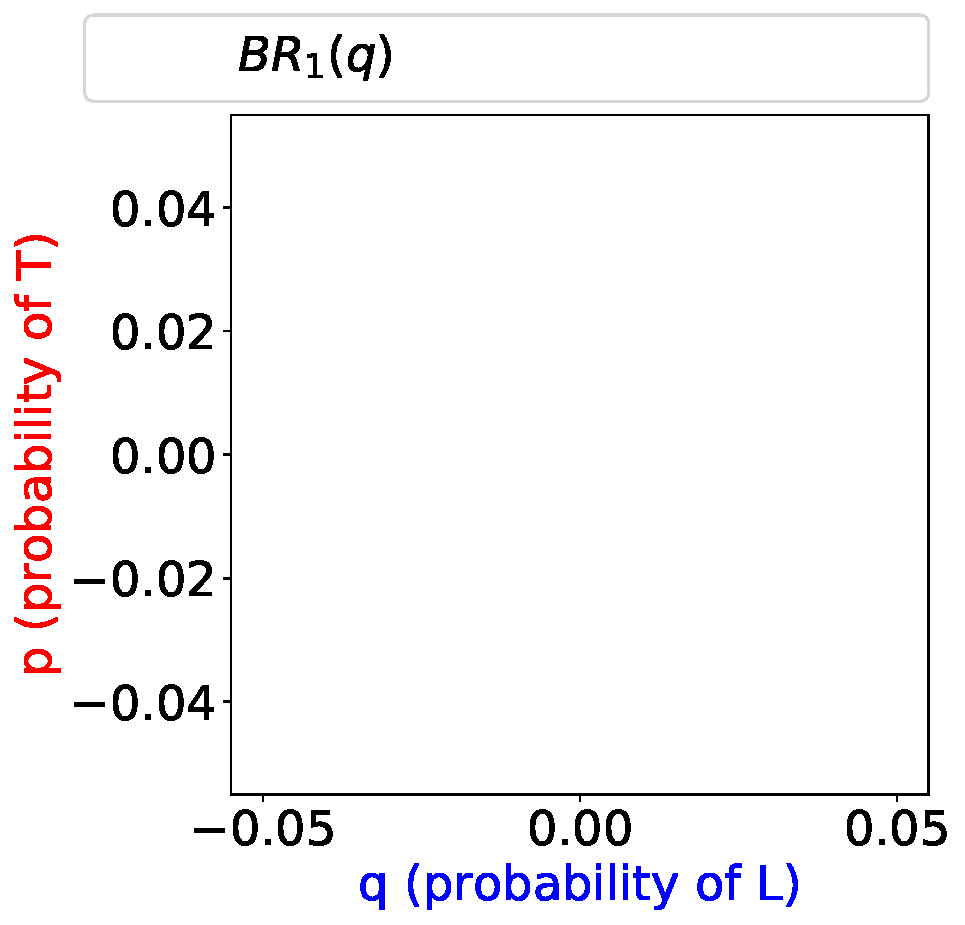
\includegraphics[width=\columnwidth]{figures/empty_plot_}
%     \textbf{\textit{Plot Alice's BR function, $\bm{p^{*}(q)}$}}
%   \vfill\null
%   \end{multicols}
% \end{frame}
% \begin{frame}{PS4, Ex. 3.b: The Focal Point (plotting BR functions)}
%   \begin{multicols}{2}
%     \begin{itemize}
%       \item[(b)] Now assume that Thomas wants to meet Alice, but Alice does not want to meet Thomas. Find all NE.
%     \end{itemize}
%     \vspace{-4pt}
%     \begin{table}
%       \begin{tabular}{cl|c|c|}
%         & \multicolumn{1}{c}{} & \multicolumn{2}{c}{\color{blue}Thomas}\\
%         \parbox[t]{1mm}{\multirow{3}{*}{\rotatebox[origin=r]{90}{\color{red}Alice}}}
%         & \multicolumn{1}{c}{} & \multicolumn{1}{c}{F (q)} & \multicolumn{1}{c}{O (1-q)} \\\cline{3-4}
%         & F (p) & -1, \textcolor{blue}{1} & \textcolor{red}{1}, -1 \\\cline{3-4}
%         & O (1-p) & \textcolor{red}{1}, -1 & -1, \textcolor{blue}{1} \\\cline{3-4}
%       \end{tabular}
%     \end{table}
%     No PSNE. Alice is indifferent for:
%     \begin{align*}
%         -q+(1-q)&=q-(1-q)\Leftrightarrow q=\frac{1}{2}
%     \end{align*}
%     Thomas is indifferent for:
%     \begin{align*}
%         p-(1-p)&=-p+(1-p)\Leftrightarrow p=\frac{1}{2}
%     \end{align*}
%     \begin{align*}
%       BR_A(q)=\left\{ \begin{array}{lcl}
%           p=1       & \text{if} & q<1/2 \\
%           p\in[0,1] & \text{if} & q=1/2 \\
%           p=0       & \text{if} & q>1/2
%       \end{array}\right. \\
%       BR_T(p)=\left\{ \begin{array}{lcl}
%           q=0       & \text{if} & p<1/2  \\
%           q\in[0,1] & \text{if} & p=1/2 \\
%           q=1       & \text{if} & p>1/2
%       \end{array}\right.
%     \end{align*}
%     \vfill\null \columnbreak
%     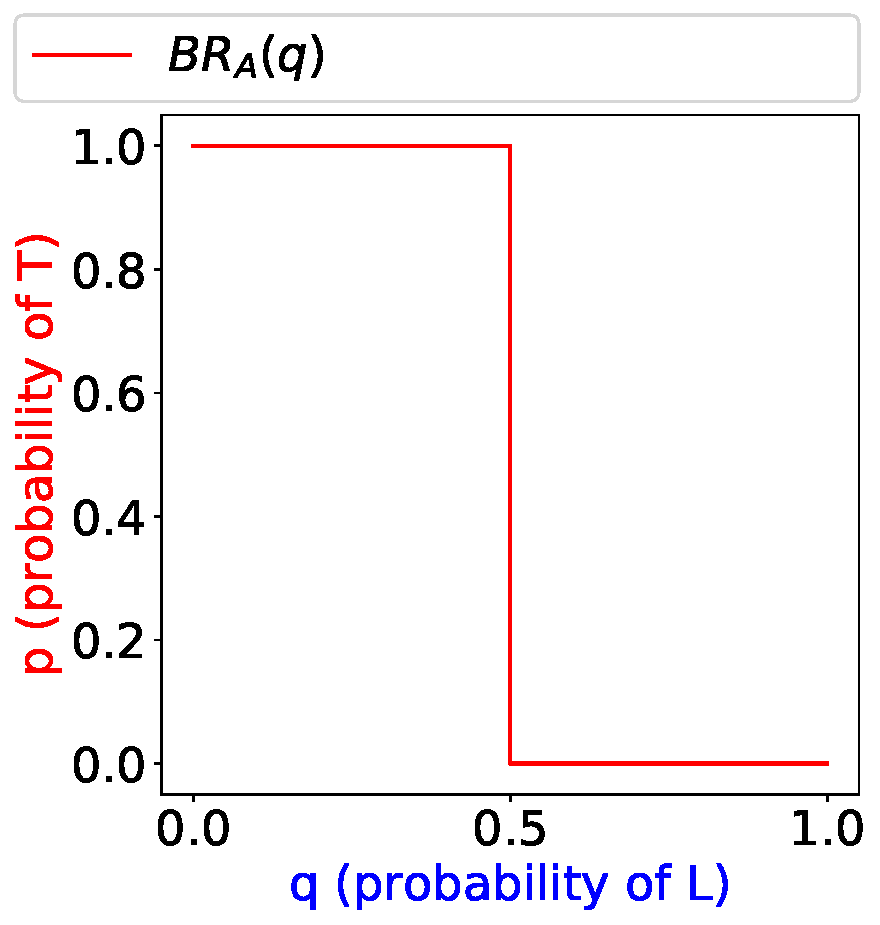
\includegraphics[width=\columnwidth]{figures/3b_}
%     \textbf{\textit{Plot Thomas' BR function, $\bm{q^{*}(p)}$}}
%   \vfill\null
%   \end{multicols}
% \end{frame}
% \begin{frame}{PS4, Ex. 3.b: The Focal Point (plotting BR functions)}
%   \begin{multicols}{2}
%     \begin{itemize}
%       \item[(b)] Now assume that Thomas wants to meet Alice, but Alice does not want to meet Thomas. Find all NE.
%     \end{itemize}
%     \vspace{-4pt}
%     \begin{table}
%       \begin{tabular}{cl|c|c|}
%         & \multicolumn{1}{c}{} & \multicolumn{2}{c}{\color{blue}Thomas}\\
%         \parbox[t]{1mm}{\multirow{3}{*}{\rotatebox[origin=r]{90}{\color{red}Alice}}}
%         & \multicolumn{1}{c}{} & \multicolumn{1}{c}{F (q)} & \multicolumn{1}{c}{O (1-q)} \\\cline{3-4}
%         & F (p) & -1, \textcolor{blue}{1} & \textcolor{red}{1}, -1 \\\cline{3-4}
%         & O (1-p) & \textcolor{red}{1}, -1 & -1, \textcolor{blue}{1} \\\cline{3-4}
%       \end{tabular}
%     \end{table}
%     No PSNE. Alice is indifferent for:
%     \begin{align*}
%         -q+(1-q)&=q-(1-q)\Leftrightarrow q=\frac{1}{2}
%     \end{align*}
%     Thomas is indifferent for:
%     \begin{align*}
%         p-(1-p)&=-p+(1-p)\Leftrightarrow p=\frac{1}{2}
%     \end{align*}
%     \begin{align*}
%       BR_A(q)=\left\{ \begin{array}{lcl}
%           p=1       & \text{if} & q<1/2 \\
%           p\in[0,1] & \text{if} & q=1/2 \\
%           p=0       & \text{if} & q>1/2
%       \end{array}\right. \\
%       BR_T(p)=\left\{ \begin{array}{lcl}
%           q=0       & \text{if} & p<1/2  \\
%           q\in[0,1] & \text{if} & p=1/2 \\
%           q=1       & \text{if} & p>1/2
%       \end{array}\right.
%     \end{align*}
%     \vfill\null \columnbreak
%     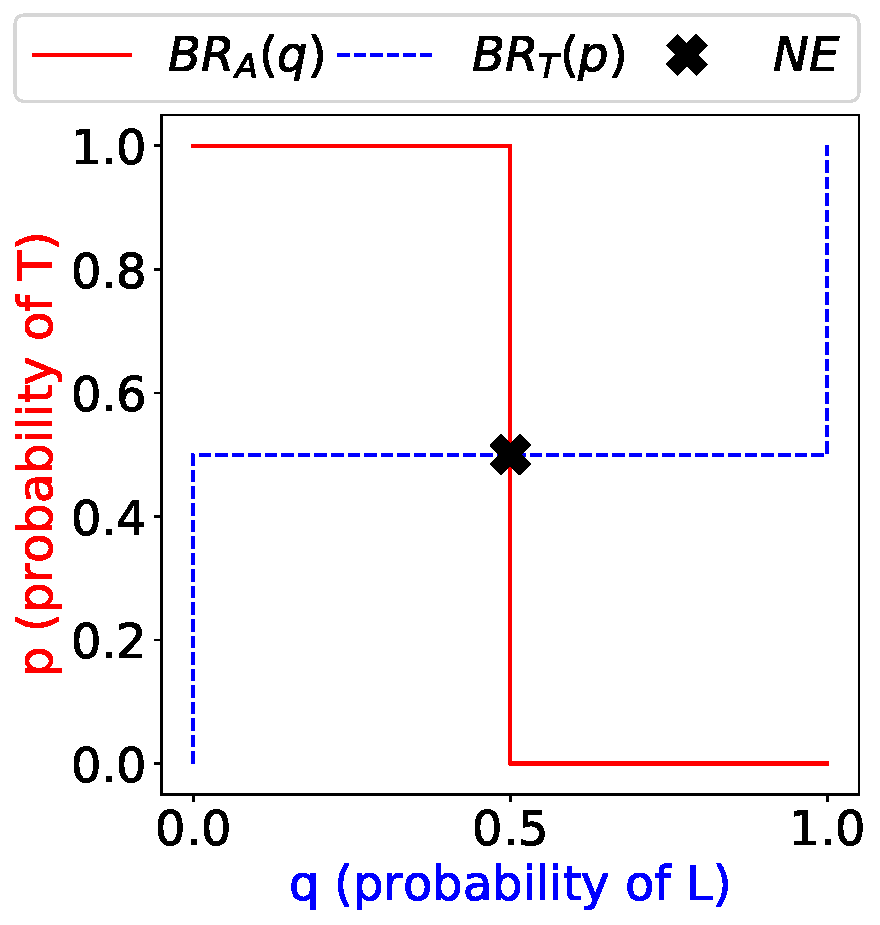
\includegraphics[width=\columnwidth]{figures/3b}
%     \textbf{\textit{Write up all NE (pure and mixed).}}
%     \begin{align*}
%       NE=(p^{*},q^{*})=
%     \end{align*}
%   \vfill\null
%   \end{multicols}
% \end{frame}
\begin{frame}{PS4, Ex. 3.b: The Focal Point (plotting BR functions)}
  \begin{multicols}{2}
    \begin{itemize}
      \item[(b)] Now assume that Thomas wants to meet Alice, but Alice does not want to meet Thomas. Find all NE.
    \end{itemize}
    \vspace{-4pt}
    \begin{table}
      \begin{tabular}{cl|c|c|}
        & \multicolumn{1}{c}{} & \multicolumn{2}{c}{\color{blue}Thomas}\\
        \parbox[t]{1mm}{\multirow{3}{*}{\rotatebox[origin=r]{90}{\color{red}Alice}}}
        & \multicolumn{1}{c}{} & \multicolumn{1}{c}{F (q)} & \multicolumn{1}{c}{O (1-q)} \\\cline{3-4}
        & F (p) & -1, \textcolor{blue}{1} & \textcolor{red}{1}, -1 \\\cline{3-4}
        & O (1-p) & \textcolor{red}{1}, -1 & -1, \textcolor{blue}{1} \\\cline{3-4}
      \end{tabular}
    \end{table}
    No PSNE. Alice is indifferent for:
    \begin{align*}
        -q+(1-q)&=q-(1-q)\Leftrightarrow q=\frac{1}{2}
    \end{align*}
    Thomas is indifferent for:
    \begin{align*}
        p-(1-p)&=-p+(1-p)\Leftrightarrow p=\frac{1}{2}
    \end{align*}
    \begin{align*}
      BR_A(q)=\left\{ \begin{array}{lcl}
          p=1       & \text{if} & q<1/2 \\
          p\in[0,1] & \text{if} & q=1/2 \\
          p=0       & \text{if} & q>1/2
      \end{array}\right. \\
      BR_T(p)=\left\{ \begin{array}{lcl}
          q=0       & \text{if} & p<1/2  \\
          q\in[0,1] & \text{if} & p=1/2 \\
          q=1       & \text{if} & p>1/2
      \end{array}\right.
    \end{align*}
    \vfill\null \columnbreak
    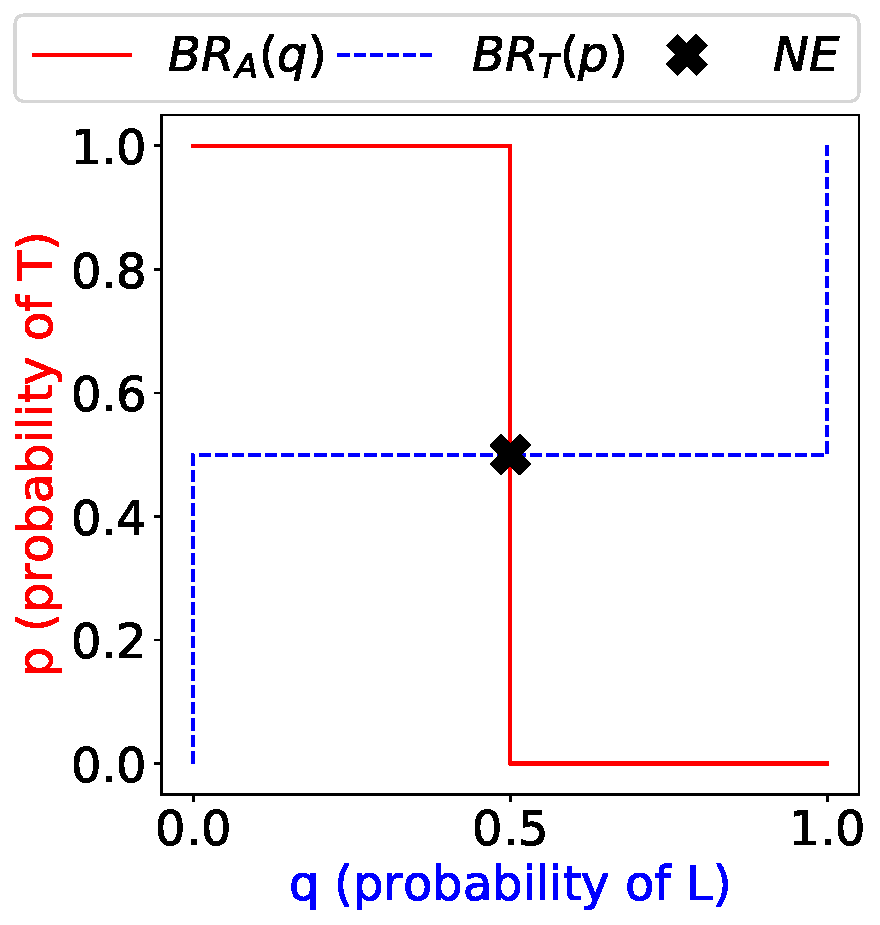
\includegraphics[width=\columnwidth]{figures/3b}
    The only NE is the Mixed Strategy NE:
    \begin{align*}
      (p^{*},q^{*})=\left(\frac{1}{2},\frac{1}{2}\right)
    \end{align*}
  \vfill\null
  \end{multicols}
\end{frame}

% \begin{frame}{PS4, Ex. 3.c: The Focal Point (plotting BR functions)}
%     \begin{itemize}
%       \item[(c)] Now assume again that Thomas and Alice both want to meet (so that payoffs are as in part (a)), but now there are $N$ bars in town, where $N$ can be very large. Show that there are $2^N-1$ equilibria (pure and mixed). Say that the bars have names: “The First Bar in Town”, “The Second Bar in Town”, and so on. Which equilibrium is the most realistic?
%     \end{itemize}
%   \vfill\null
%   \end{frame}
% \begin{frame}{PS4, Ex. 3.c: The Focal Point (plotting BR functions)}
%     \begin{itemize}
%       \item[(c)] Now assume again that Thomas and Alice both want to meet (so that payoffs are as in part (a)), but now there are $N$ bars in town, where $N$ can be very large. Show that there are $2^N-1$ equilibria (pure and mixed). Say that the bars have names: “The First Bar in Town”, “The Second Bar in Town”, and so on.
%     \end{itemize}
%   \begin{multicols}{2}
%     \textbf{For N=2:} We have $3=2^N-1$ equilibria:
%     \begin{align*}
%       (p^{*},q^{*})&=\left\{(0,0);(1,1);\left(\frac{1}{2},\frac{1}{2}\right)\right\}
%     \end{align*}
%   \vfill\null \columnbreak
%     \vspace{-12pt}
%     \begin{table}
%       \begin{tabular}{cl|c|c|}
%         & \multicolumn{1}{c}{} & \multicolumn{2}{c}{\color{blue}Thomas}\\
%         \parbox[t]{1mm}{\multirow{3}{*}{\rotatebox[origin=r]{90}{\color{red}Alice}}}
%         & \multicolumn{1}{c}{} & \multicolumn{1}{c}{$Bar_1$ (q)} & \multicolumn{1}{c}{$Bar_2$ (1-q)} \\\cline{3-4}
%         & $Bar_1$ (p) & \textcolor{red}{1}, \textcolor{blue}{1} & 0, 0 \\\cline{3-4}
%         & $Bar_2$ (1-p) & 0, 0 & \textcolor{red}{1}, \textcolor{blue}{1} \\\cline{3-4}
%       \end{tabular}
%     \end{table}
%   \vfill\null
%   \end{multicols}
%     \textbf{\textit{What about N=3?}}\\\bigskip
%     \textbf{\textit{And any N?}}
% \end{frame}
% \begin{frame}{PS4, Ex. 3.c: The Focal Point (plotting BR functions)}
%     \begin{itemize}
%       \item[(c)] Now assume again that Thomas and Alice both want to meet (so that payoffs are as in part (a)), but now there are $N$ bars in town, where $N$ can be very large. Show that there are $2^N-1$ equilibria (pure and mixed). Say that the bars have names: “The First Bar in Town”, “The Second Bar in Town”, and so on.
%     \end{itemize}
%   \begin{multicols}{2}
%     \textbf{For N=2:} We have $3=2^N-1$ equilibria:
%     \begin{align*}
%       (p^{*},q^{*})&=\left\{(0,0);(1,1);\left(\frac{1}{2},\frac{1}{2}\right)\right\}
%     \end{align*}
%   \vfill\null \columnbreak
%     \vspace{-12pt}
%     \begin{table}
%       \begin{tabular}{cl|c|c|}
%         & \multicolumn{1}{c}{} & \multicolumn{2}{c}{\color{blue}Thomas}\\
%         \parbox[t]{1mm}{\multirow{3}{*}{\rotatebox[origin=r]{90}{\color{red}Alice}}}
%         & \multicolumn{1}{c}{} & \multicolumn{1}{c}{$Bar_1$ (q)} & \multicolumn{1}{c}{$Bar_2$ (1-q)} \\\cline{3-4}
%         & $Bar_1$ (p) & \textcolor{red}{1}, \textcolor{blue}{1} & 0, 0 \\\cline{3-4}
%         & $Bar_2$ (1-p) & 0, 0 & \textcolor{red}{1}, \textcolor{blue}{1} \\\cline{3-4}
%       \end{tabular}
%     \end{table}
%   \vfill\null
%   \end{multicols}
%     \textbf{\textit{What about N=3?}}
%     \vspace{-12pt}
%     \begin{table}
%       \begin{tabular}{cl|c|c|c|}
%         & \multicolumn{1}{c}{} & \multicolumn{3}{c}{\color{blue}Thomas}\\
%         & \multicolumn{1}{c}{} & \multicolumn{1}{c}{$Bar_1$ ($q_1$)} & \multicolumn{1}{c}{$Bar_2$ ($q_2$)} & \multicolumn{1}{c}{$Bar_3$ (1-$q_1$-$q_2$)} \\\cline{3-5}
%         \parbox[t]{1mm}{\multirow{3}{*}{\rotatebox[origin=c]{90}{\color{red}Alice}}}
%         & $Bar_1$ ($p_1$) & \textcolor{red}{1}, \textcolor{blue}{1} & 0, 0 & 0, 0 \\\cline{3-5}
%         & $Bar_2$ ($p_2$) & 0, 0 & \textcolor{red}{1}, \textcolor{blue}{1} & 0, 0 \\\cline{3-5}
%         & $Bar_3$ (1-$p_1$-$p_2$) & 0, 0 & 0, 0 & \textcolor{red}{1}, \textcolor{blue}{1} \\\cline{3-5}
%       \end{tabular}
%     \end{table}
%     \textbf{\textit{And any N?}}
% \end{frame}
% \begin{frame}{PS4, Ex. 3.c: The Focal Point (plotting BR functions)}
%     \begin{itemize}
%       \item[(c)] Now assume again that Thomas and Alice both want to meet (so that payoffs are as in part (a)), but now there are $N$ bars in town, where $N$ can be very large. Show that there are $2^N-1$ equilibria (pure and mixed). Say that the bars have names: “The First Bar in Town”, “The Second Bar in Town”, and so on.
%     \end{itemize}
%     \vspace{-6pt}
%   \begin{multicols}{2}
%     \textbf{For N=2:} We have $3=2^N-1$ equilibria:
%     \begin{align*}
%       (p^{*},q^{*})&=\left\{(0,0);(1,1);\left(\frac{1}{2},\frac{1}{2}\right)\right\}
%     \end{align*}
%   \vfill\null \columnbreak
%     \vspace{-12pt}
%     \begin{table}
%       \begin{tabular}{cl|c|c|}
%         & \multicolumn{1}{c}{} & \multicolumn{2}{c}{\color{blue}Thomas}\\
%         \parbox[t]{1mm}{\multirow{3}{*}{\rotatebox[origin=r]{90}{\color{red}Alice}}}
%         & \multicolumn{1}{c}{} & \multicolumn{1}{c}{$Bar_1$ (q)} & \multicolumn{1}{c}{$Bar_2$ (1-q)} \\\cline{3-4}
%         & $Bar_1$ (p) & \textcolor{red}{1}, \textcolor{blue}{1} & 0, 0 \\\cline{3-4}
%         & $Bar_2$ (1-p) & 0, 0 & \textcolor{red}{1}, \textcolor{blue}{1} \\\cline{3-4}
%       \end{tabular}
%     \end{table}
%   \vfill\null
%   \end{multicols}
%     \vspace{-20pt}
%     \textbf{For N=3:} We have $7=2^N-1$ equilibria, $(p_1^{*},p_2^{*},q_1^{*},q_2^{*})$:
%     \begin{align*}
%       \left\{(0,0,0,0);(0,1,0,1);(1,0,1,0)
%       ;\left(\frac{1}{2},\frac{1}{2},\frac{1}{2},\frac{1}{2}\right)
%       ;\left(\frac{1}{2},0,\frac{1}{2},0\right)
%       ;\left(0,\frac{1}{2},0,\frac{1}{2}\right)
%       ;\left(\frac{1}{3},\frac{1}{3},\frac{1}{3},\frac{1}{3}\right)
%       \right\}
%     \end{align*}
%     \vspace{-12pt}
%     \begin{table}
%       \begin{tabular}{cl|c|c|c|}
%         & \multicolumn{1}{c}{} & \multicolumn{3}{c}{\color{blue}Thomas}\\
%         & \multicolumn{1}{c}{} & \multicolumn{1}{c}{$Bar_1$ ($q_1$)} & \multicolumn{1}{c}{$Bar_2$ ($q_2$)} & \multicolumn{1}{c}{$Bar_3$ (1-$q_1$-$q_2$)} \\\cline{3-5}
%         \parbox[t]{1mm}{\multirow{3}{*}{\rotatebox[origin=c]{90}{\color{red}Alice}}}
%         & $Bar_1$ ($p_1$) & \textcolor{red}{1}, \textcolor{blue}{1} & 0, 0 & 0, 0 \\\cline{3-5}
%         & $Bar_2$ ($p_2$) & 0, 0 & \textcolor{red}{1}, \textcolor{blue}{1} & 0, 0 \\\cline{3-5}
%         & $Bar_3$ (1-$p_1$-$p_2$) & 0, 0 & 0, 0 & \textcolor{red}{1}, \textcolor{blue}{1} \\\cline{3-5}
%       \end{tabular}
%     \end{table}
%     \textbf{\textit{What about any N?}}
% \end{frame}
% \begin{frame}{PS4, Ex. 3.c: The Focal Point (plotting BR functions)}
%     \begin{itemize}
%       \item[(c)] Which equilibrium is the most realistic?
%     \end{itemize}
%     \textbf{For N=3:} We have $7=2^N-1$ equilibria, $(p_1^{*},p_2^{*},q_1^{*},q_2^{*})$:
%     \begin{align*}
%       \left\{(0,0,0,0);(0,1,0,1);(1,0,1,0)
%       ;\left(\frac{1}{2},\frac{1}{2},\frac{1}{2},\frac{1}{2}\right)
%       ;\left(\frac{1}{2},0,\frac{1}{2},0\right)
%       ;\left(0,\frac{1}{2},0,\frac{1}{2}\right)
%       ;\left(\frac{1}{3},\frac{1}{3},\frac{1}{3},\frac{1}{3}\right)
%       \right\}
%     \end{align*}
%     \vspace{-18pt}
%     \begin{table}
%       \begin{tabular}{cl|c|c|c|}
%         & \multicolumn{1}{c}{} & \multicolumn{3}{c}{\color{blue}Thomas}\\
%         & \multicolumn{1}{c}{} & \multicolumn{1}{c}{$Bar_1$ ($q_1$)} & \multicolumn{1}{c}{$Bar_2$ ($q_2$)} & \multicolumn{1}{c}{$Bar_3$ (1-$q_1$-$q_2$)} \\\cline{3-5}
%         \parbox[t]{1mm}{\multirow{3}{*}{\rotatebox[origin=c]{90}{\color{red}Alice}}}
%         & $Bar_1$ ($p_1$) & \textcolor{red}{1}, \textcolor{blue}{1} & 0, 0 & 0, 0 \\\cline{3-5}
%         & $Bar_2$ ($p_2$) & 0, 0 & \textcolor{red}{1}, \textcolor{blue}{1} & 0, 0 \\\cline{3-5}
%         & $Bar_3$ (1-$p_1$-$p_2$) & 0, 0 & 0, 0 & \textcolor{red}{1}, \textcolor{blue}{1} \\\cline{3-5}
%       \end{tabular}
%     \end{table}
%     \textbf{\textit{Look at the expected payoffs from the pure and mixed equilibria when N=3...}}
% \end{frame}
% \begin{frame}{PS4, Ex. 3.c: The Focal Point (plotting BR functions)}
%     \begin{itemize}
%       \item[(c)] Which equilibrium is the most realistic?
%     \end{itemize}
%     \textbf{For N=3:} We have $7=2^N-1$ equilibria, $(p_1^{*},p_2^{*},q_1^{*},q_2^{*})$:
%     \begin{align*}
%       \left\{(0,0,0,0);(0,1,0,1);(1,0,1,0)
%       ;\left(\frac{1}{2},\frac{1}{2},\frac{1}{2},\frac{1}{2}\right)
%       ;\left(\frac{1}{2},0,\frac{1}{2},0\right)
%       ;\left(0,\frac{1}{2},0,\frac{1}{2}\right)
%       ;\left(\frac{1}{3},\frac{1}{3},\frac{1}{3},\frac{1}{3}\right)
%       \right\}
%     \end{align*}
%     \vspace{-18pt}
%     \begin{table}
%       \begin{tabular}{cl|c|c|c|}
%         & \multicolumn{1}{c}{} & \multicolumn{3}{c}{\color{blue}Thomas}\\
%         & \multicolumn{1}{c}{} & \multicolumn{1}{c}{$Bar_1$ ($q_1$)} & \multicolumn{1}{c}{$Bar_2$ ($q_2$)} & \multicolumn{1}{c}{$Bar_3$ (1-$q_1$-$q_2$)} \\\cline{3-5}
%         \parbox[t]{1mm}{\multirow{3}{*}{\rotatebox[origin=c]{90}{\color{red}Alice}}}
%         & $Bar_1$ ($p_1$) & \textcolor{red}{1}, \textcolor{blue}{1} & 0, 0 & 0, 0 \\\cline{3-5}
%         & $Bar_2$ ($p_2$) & 0, 0 & \textcolor{red}{1}, \textcolor{blue}{1} & 0, 0 \\\cline{3-5}
%         & $Bar_3$ (1-$p_1$-$p_2$) & 0, 0 & 0, 0 & \textcolor{red}{1}, \textcolor{blue}{1} \\\cline{3-5}
%       \end{tabular}
%     \end{table}
%     In the three PSNE, the expected payoffs are: $\left(E[u_A|q_1^{*},q_2^{*})],E[u_T|p_1^{*},p_2^{*})]\right)=$
%     \begin{align*}
%       \left\{(1-q_1-q_2,1-p_1-p_2);(q_2,p_2);(q_1,p_1)\right\}\sim
%       \left\{(1,1);(1,1);(1,1)\right\}
%     \end{align*}
%     \textbf{\textit{What are the expected payoffs In the four MSNE?}}
% \end{frame}
% \begin{frame}{PS4, Ex. 3.c: The Focal Point (plotting BR functions)}
%     \begin{itemize}
%       \item[(c)] Which equilibrium is the most realistic?
%     \end{itemize}
%     \textbf{For N=3:} We have $7=2^N-1$ equilibria, $(p_1^{*},p_2^{*},q_1^{*},q_2^{*})$:
%     \begin{align*}
%       \left\{(0,0,0,0);(0,1,0,1);(1,0,1,0)
%       ;\left(\frac{1}{2},\frac{1}{2},\frac{1}{2},\frac{1}{2}\right)
%       ;\left(\frac{1}{2},0,\frac{1}{2},0\right)
%       ;\left(0,\frac{1}{2},0,\frac{1}{2}\right)
%       ;\left(\frac{1}{3},\frac{1}{3},\frac{1}{3},\frac{1}{3}\right)
%       \right\}
%     \end{align*}
%     \vspace{-12pt}
%     \begin{table}
%       \begin{tabular}{cl|c|c|c|}
%         & \multicolumn{1}{c}{} & \multicolumn{3}{c}{\color{blue}Thomas}\\
%         & \multicolumn{1}{c}{} & \multicolumn{1}{c}{$Bar_1$ ($q_1$)} & \multicolumn{1}{c}{$Bar_2$ ($q_2$)} & \multicolumn{1}{c}{$Bar_3$ (1-$q_1$-$q_2$)} \\\cline{3-5}
%         \parbox[t]{1mm}{\multirow{3}{*}{\rotatebox[origin=c]{90}{\color{red}Alice}}}
%         & $Bar_1$ ($p_1$) & \textcolor{red}{1}, \textcolor{blue}{1} & 0, 0 & 0, 0 \\\cline{3-5}
%         & $Bar_2$ ($p_2$) & 0, 0 & \textcolor{red}{1}, \textcolor{blue}{1} & 0, 0 \\\cline{3-5}
%         & $Bar_3$ (1-$p_1$-$p_2$) & 0, 0 & 0, 0 & \textcolor{red}{1}, \textcolor{blue}{1} \\\cline{3-5}
%       \end{tabular}
%     \end{table}
%     In the three PSNE, the expected payoffs are: $\left(E[u_A|q_1^{*},q_2^{*})],E[u_T|p_1^{*},p_2^{*})]\right)=$
%     \begin{align*}
%       \left\{(1-q_1-q_2,1-p_1-p_2);(q_2,p_2);(q_1,p_1)\right\}\sim
%       \left\{(1,1);(1,1);(1,1)\right\}
%     \end{align*}
%     In the four MSNE, the expected payoffs are: $\left(E[u_A|q_1^{*},q_2^{*})],E[u_T|p_1^{*},p_2^{*})]\right)=$
%     \begin{align*}
%      &\left\{\left(\frac{q_1+q_2}{2},\frac{p_1+p_2}{2}\right)
%       ;\left(\frac{1-q_2}{2},\frac{1-p_2}{2}\right)
%       ;\left(\frac{1-q_1}{2},\frac{1-p_1}{2}\right)
%       ;\left(\frac{1}{3},\frac{1}{3}\right)\right\} \\
%      \sim
%      &\left\{\left(\frac{1}{2},\frac{1}{2}\right)
%       ;\left(\frac{1}{2},\frac{1}{2}\right)
%       ;\left(\frac{1}{2},\frac{1}{2}\right)
%       ;\left(\frac{1}{3},\frac{1}{3}\right)\right\}
%     \end{align*}
%     \textbf{\textit{Which equilibria are the most realistic - and which is the least realistic?}}
% \end{frame}
\begin{frame}{PS4, Ex. 3.c: The Focal Point (plotting BR functions)}
    \begin{itemize}
      \item[(c)] Which equilibrium is the most realistic?
    \end{itemize}
    \textbf{For N=3:} We have $7=2^N-1$ equilibria, $(p_1^{*},p_2^{*},q_1^{*},q_2^{*})$:
    \begin{align*}
      \left\{(0,0,0,0);(0,1,0,1);(1,0,1,0)
      ;\left(\frac{1}{2},\frac{1}{2},\frac{1}{2},\frac{1}{2}\right)
      ;\left(\frac{1}{2},0,\frac{1}{2},0\right)
      ;\left(0,\frac{1}{2},0,\frac{1}{2}\right)
      ;\left(\frac{1}{3},\frac{1}{3},\frac{1}{3},\frac{1}{3}\right)
      \right\}
    \end{align*}
    \vspace{-12pt}
    \begin{table}
      \begin{tabular}{cl|c|c|c|}
        & \multicolumn{1}{c}{} & \multicolumn{3}{c}{\color{blue}Thomas}\\
        & \multicolumn{1}{c}{} & \multicolumn{1}{c}{$Bar_1$ ($q_1$)} & \multicolumn{1}{c}{$Bar_2$ ($q_2$)} & \multicolumn{1}{c}{$Bar_3$ (1-$q_1$-$q_2$)} \\\cline{3-5}
        \parbox[t]{1mm}{\multirow{3}{*}{\rotatebox[origin=c]{90}{\color{red}Alice}}}
        & $Bar_1$ ($p_1$) & \textcolor{red}{1}, \textcolor{blue}{1} & 0, 0 & 0, 0 \\\cline{3-5}
        & $Bar_2$ ($p_2$) & 0, 0 & \textcolor{red}{1}, \textcolor{blue}{1} & 0, 0 \\\cline{3-5}
        & $Bar_3$ (1-$p_1$-$p_2$) & 0, 0 & 0, 0 & \textcolor{red}{1}, \textcolor{blue}{1} \\\cline{3-5}
      \end{tabular}
    \end{table}
    In the three PSNE, the expected payoffs are: $\left(E[u_A|q_1^{*},q_2^{*})],E[u_T|p_1^{*},p_2^{*})]\right)=$
    \begin{align*}
      \left\{(1-q_1-q_2,1-p_1-p_2);(q_2,p_2);(q_1,p_1)\right\}\sim
      \left\{(1,1);(1,1);(1,1)\right\}
    \end{align*}
    In the four MSNE, the expected payoffs are: $\left(E[u_A|q_1^{*},q_2^{*})],E[u_T|p_1^{*},p_2^{*})]\right)=$
    \begin{align*}
     &\left\{\left(\frac{q_1+q_2}{2},\frac{p_1+p_2}{2}\right)
      ;\left(\frac{1-q_2}{2},\frac{1-p_2}{2}\right)
      ;\left(\frac{1-q_1}{2},\frac{1-p_1}{2}\right)
      ;\left(\frac{1}{3},\frac{1}{3}\right)\right\} \\
     \sim
     &\left\{\left(\frac{1}{2},\frac{1}{2}\right)
      ;\left(\frac{1}{2},\frac{1}{2}\right)
      ;\left(\frac{1}{2},\frac{1}{2}\right)
      ;\left(\frac{1}{3},\frac{1}{3}\right)\right\}
    \end{align*}
    PSNE are the most realistic due to higher payoffs. Due to coordination issues, the expected payoffs are reciprocal to the number of actions that a MSNE is split between.
\end{frame}

\end{document}
